% ==============================================================================
% Phân mục 07: Kết quả thực nghiệm (Results) – THÀNH VIÊN 1 (+ Thành viên 2 phần DCA/fairness)
% Mọi con số được \input từ generated/*.tex (sinh bởi scripts/export_latex_tables.py từ
% results/registry.json). KHÔNG gõ tay số liệu vào file này.
% ==============================================================================
\section{Kết Quả (Results)}
\label{sec:empirical_results}

\subsection{RQ1 -- So sánh công bằng giữa các mô hình}
Bảng~\ref{tab:rq1} trình bày kết quả của mười mô hình trên tập kiểm thử strict ($N=\testN$). Ba quan sát chính:
\begin{enumerate}[leftmargin=1.8em, itemsep=0.2em]
  \item \textbf{Mô hình đơn phương thức mạnh nhất là Bio\_ClinicalBERT fine-tune} (macro AUROC \aucBertFT{} $\pm$ \aucsdBertFT{}), cao hơn mọi mô hình chỉ dùng dữ liệu bảng. Ensemble trung bình xác suất CatBoost + BERT-FT đạt \aucEnsemble{} $\pm$ \aucsdEnsemble{}.
  \item \textbf{Cross-attention đóng băng (mô hình triển khai)} đạt \aucXattn{} $\pm$ \aucsdXattn{}: cao hơn có ý nghĩa thống kê so với CatBoost ($\Delta=\deltaCatBoost$, $p_{\text{Holm}}=\pCatBoost$), TF-IDF + LR, BERT đóng băng và concat fusion, nhưng \emph{không khác biệt} so với Logistic Regression ($\Delta=\deltaLRTab{}$, $p_{\text{Holm}}=\pLRTab$) và FT-Transformer chỉ dùng dữ liệu bảng ($\Delta=\deltaFTT{}$, $p_{\text{Holm}}=\pFTT$), và \emph{thấp hơn có ý nghĩa} so với BERT-FT ($\Delta=\deltaBertFT{}$ \deltaciBertFT, $p_{\text{Holm}}=\pBertFT$) và ensemble ($\Delta=\deltaEnsemble{}$, $p_{\text{Holm}}=\pEnsemble$).
  \item \textbf{Fine-tune khối BERT cuối trong mô hình dung hợp không cải thiện}: cross-attention fine-tune đạt \aucXattnFT{} $\pm$ \aucsdXattnFT{}, không khác mô hình triển khai ($p_{\text{Holm}}=\pXattnFT$). Mô hình dung hợp có độ biến thiên giữa các seed lớn hơn mô hình đơn phương thức (concat: SD \aucsdConcat{}); vì seed đại diện được chọn theo NLL validation, khoảng cách ở cột $\Delta$ của concat lớn hơn chênh lệch trung bình qua seed.
\end{enumerate}
Như vậy, trên tập test strict, giả thuyết ``dung hợp chú ý chéo vượt mô hình đơn phương thức tốt nhất'' \textbf{không được ủng hộ}. Tuy nhiên, phân tích độ nhạy post-hoc bằng 5-fold grouped CV (Bảng~\ref{tab:generalization}) cho bức tranh khác: cross-attention đạt \cvXattn{} $\pm$ \cvsdXattn{} và là mô hình \emph{ổn định nhất} qua các fold, trong khi BERT-FT đạt \cvBertFT{} $\pm$ \cvsdBertFT{} (fold kém nhất \cvminBertFT) và ensemble \cvEnsemble{} $\pm$ \cvsdEnsemble. Ưu thế của BERT-FT trên tập test strict vì vậy không bền khi tập test gồm các bệnh nhân gốc khác; kết luận RQ1 phụ thuộc vào cách chia dữ liệu và cần được kiểm chứng trên dữ liệu thật.

% AUTO-GENERATED by scripts/export_latex_tables.py from results/registry.json. Do not edit.
\begin{table}[htbp]\centering\scriptsize
\caption{RQ1 -- So sánh công bằng trên tập kiểm thử strict ($N=302$). AUROC/F1/ECE: trung bình $\pm$ SD qua seed (xác suất đã hiệu chuẩn nhiệt độ trên validation). CI 95\%: bootstrap theo bản ghi ($B=2000$) trên seed có NLL validation thấp nhất -- các bản ghi chung bệnh nhân Synthea gốc nên CI hẹp hơn độ bất định thực. $\Delta$: Cross-attention (đóng băng) trừ mô hình so sánh; $p$ hiệu chỉnh Holm.}
\label{tab:rq1}
\begin{tabular}{@{}llccccc@{}}\toprule
Nhóm & Mô hình & AUROC (TB $\pm$ SD, $n$ seed) & AUROC seed đại diện [CI 95\%] & Macro-F1 & ECE & $\Delta$AUROC [CI 95\%], $p_{\text{Holm}}$ \\ \midrule
Chỉ dữ liệu bảng & Logistic Regression & 0.945 (1) & 0.945 [0.927; 0.962] & 0.669 & 0.078 & +0.013 [-0.005; 0.033], 0.456 \\
 & CatBoost & 0.925 $\pm$ 0.003 (5) & 0.926 [0.904; 0.945] & 0.647 $\pm$ 0.030 & 0.061 & +0.033 [0.014; 0.053], 0.010 \\
 & FT-Transformer & 0.929 $\pm$ 0.019 (5) & 0.949 [0.931; 0.964] & 0.732 $\pm$ 0.090 & 0.092 & +0.010 [-0.008; 0.027], 0.516 \\
\midrule
Chỉ văn bản & TF-IDF + LR & 0.917 (1) & 0.917 [0.893; 0.941] & 0.674 & 0.094 & +0.041 [0.019; 0.065], 0.009 \\
 & Bio\_ClinicalBERT (đóng băng) & 0.899 $\pm$ 0.027 (5) & 0.904 [0.879; 0.927] & 0.592 $\pm$ 0.115 & 0.116 & +0.054 [0.029; 0.080], 0.009 \\
 & Bio\_ClinicalBERT (fine-tune) & 0.975 $\pm$ 0.004 (5) & 0.978 [0.969; 0.987] & 0.843 $\pm$ 0.029 & 0.072 & -0.020 [-0.033; -0.008], 0.012 \\
\midrule
Dung hợp & Concat fusion & 0.929 $\pm$ 0.021 (5) & 0.892 [0.870; 0.913] & 0.742 $\pm$ 0.109 & 0.116 & +0.066 [0.048; 0.086], 0.009 \\
 & \textbf{Cross-attention (đóng băng)} & 0.956 $\pm$ 0.008 (5) & 0.958 [0.943; 0.972] & 0.691 $\pm$ 0.021 & 0.081 & (tham chiếu) \\
 & Cross-attention (fine-tune) & 0.961 $\pm$ 0.015 (5) & 0.958 [0.945; 0.970] & 0.726 $\pm$ 0.116 & 0.106 & +0.000 [-0.010; 0.010], 0.930 \\
 & Ensemble CatBoost + BERT-FT & 0.978 $\pm$ 0.003 (5) & 0.982 [0.973; 0.990] & 0.801 $\pm$ 0.052 & 0.116 & -0.024 [-0.035; -0.013], 0.009 \\
\bottomrule\end{tabular}\end{table}


\subsection{RQ2 -- Tín hiệu văn bản đến từ đâu}
Bảng~\ref{tab:rq2} và Hình~\ref{fig:rq2} cho thấy hiệu năng của các mô hình chỉ dùng văn bản phụ thuộc gần như hoàn toàn vào các giá trị số nằm trong ghi chú. Khi mọi con số bị thay bằng \texttt{<NUM>}, AUROC của BERT-FT giảm từ \rqtwoBertFTFull{} xuống \rqtwoBertFTNumMasked{} và của TF-IDF + LR từ \rqtwoTfidfFull{} xuống \rqtwoTfidfNumMasked{}; khi chỉ giữ phần tự sự (lý do khám, bệnh sử, thuốc), BERT-FT còn \rqtwoBertFTNarrative{}. Đáng chú ý, khi bỏ sinh hiệu/xét nghiệm nhưng vẫn giữ tuổi trong tiêu đề và bệnh sử (``Age: 97'', ``97yo''), BERT-FT vẫn đạt \rqtwoBertFTNoVitals{} -- phù hợp với việc tuổi gần như tự phân tách các lớp trong đoàn hệ này (Mục~\ref{sec:clinical_cohort}); chỉ khi \emph{mọi} con số (kể cả tuổi) bị che thì tín hiệu văn bản mới biến mất. Ngược lại, cross-attention giữ AUROC \rqtwoXattnNumMasked{} (che số) và \rqtwoXattnNarrative{} (chỉ tự sự), tương đương các mô hình chỉ dùng dữ liệu bảng -- tức mô hình dung hợp dựa vào nhánh bảng khi văn bản không còn thông tin số. Nói cách khác, trong dữ liệu bán tổng hợp này, ghi chú lâm sàng chủ yếu \emph{mã hoá lại} sinh hiệu và xét nghiệm, và lợi thế của BERT-FT so với mô hình bảng đến từ việc đọc các con số đó cùng ngữ cảnh định dạng của ghi chú, không phải từ mô tả triệu chứng.

% AUTO-GENERATED by scripts/export_latex_tables.py from results/registry.json. Do not edit.
\begin{table}[htbp]\centering\small
\caption{RQ2 -- Phân rã tín hiệu văn bản: macro AUROC trên test strict theo biến thể ghi chú (trung bình 3 seed; TF-IDF tất định). Tham chiếu chỉ dữ liệu bảng: LR 0.945, CatBoost 0.925.}
\label{tab:rq2}
\begin{tabular}{@{}lcccc@{}}\toprule
Biến thể ghi chú & TF-IDF+LR & BERT đóng băng & BERT fine-tune & Cross-attention \\ \midrule
Ghi chú gốc & 0.917 & 0.895 $\pm$ 0.029 & 0.974 $\pm$ 0.004 & 0.954 $\pm$ 0.008 \\
Che mọi con số & 0.541 & 0.655 $\pm$ 0.049 & 0.679 $\pm$ 0.002 & 0.920 $\pm$ 0.025 \\
Bỏ sinh hiệu/xét nghiệm & 0.885 & 0.923 $\pm$ 0.011 & 0.905 $\pm$ 0.046 & 0.965 $\pm$ 0.012 \\
Chỉ phần tự sự & 0.826 & 0.777 $\pm$ 0.011 & 0.776 $\pm$ 0.060 & 0.917 $\pm$ 0.022 \\
\bottomrule\end{tabular}\end{table}


\begin{figure}[htbp]
  \centering
  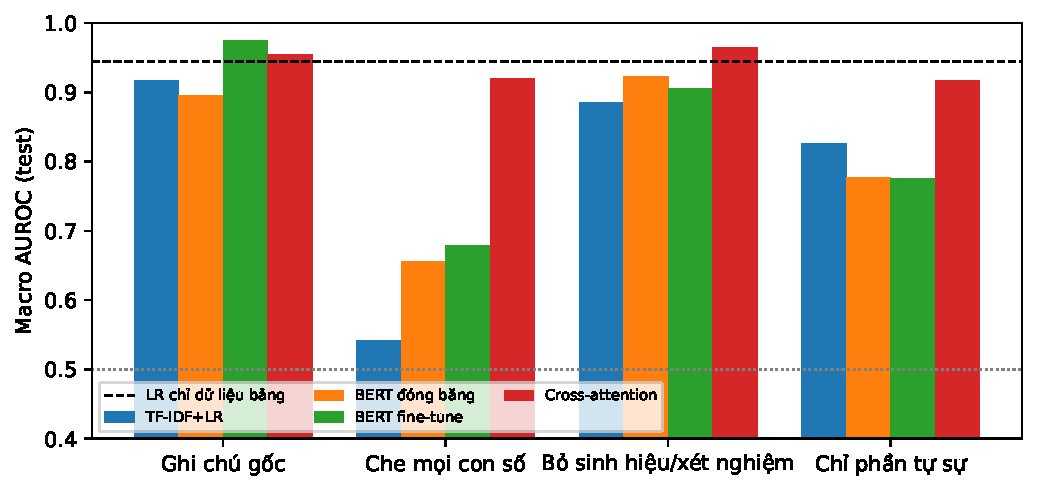
\includegraphics[width=0.85\linewidth]{figures/generated/fig_rq2_text_decomposition.pdf}
  \caption{RQ2 -- Macro AUROC theo biến thể ghi chú. Đường đứt nét: Logistic Regression chỉ dùng dữ liệu bảng; đường chấm: đoán ngẫu nhiên.}
  \label{fig:rq2}
\end{figure}

\subsection{RQ3 -- Khi nào dung hợp có ích (mô phỏng)}
\IfFileExists{generated/tab_rq3.tex}{%
Bảng~\ref{tab:rq3} và Hình~\ref{fig:rq3} trình bày kết quả mô phỏng. Đây là \textbf{thí nghiệm mô phỏng cơ chế}: câu triệu chứng đặc hiệu do nhóm nghiên cứu chèn vào ghi chú đã che số, nên kết quả chỉ cho biết điều kiện để kiến trúc khai thác được thông tin bổ trợ, không phản ánh hiệu năng lâm sàng. % AUTO-GENERATED by scripts/export_latex_tables.py from results/registry.json. Do not edit.
Khi văn bản không có tín hiệu riêng ($\rho=0$) và dữ liệu bảng không nhiễu ($\sigma=0$), cross-attention đạt 0.933 so với 0.939 của mô hình đơn phương thức tốt hơn ($\Delta=-0.005$). Khi mọi ca có tín hiệu văn bản ($\rho=1$) và dữ liệu bảng nhiễu mạnh ($\sigma=1$), $\Delta=+0.039$. $\Delta$ lớn nhất là +0.060 tại $(\rho,\sigma)=(0.25,1)$ và nhỏ nhất là -0.014 tại $(0,0.5)$; 9/15 cấu hình có $\Delta>0.01$.

% AUTO-GENERATED by scripts/export_latex_tables.py from results/registry.json. Do not edit.
\begin{table}[htbp]\centering\small
\caption{RQ3 -- \textbf{Mô phỏng} bổ trợ có kiểm soát: macro AUROC (trung bình 2 seed). $\rho$: tỷ lệ ca có câu triệu chứng đặc hiệu trong ghi chú đã che số; $\sigma$: nhiễu Gauss trên biến số (bội số SD). $\Delta$ = cross-attention trừ mô hình đơn phương thức tốt hơn.}
\label{tab:rq3}
\begin{tabular}{@{}cccccc@{}}\toprule
$\rho$ & $\sigma$ & Bảng & Văn bản & Cross-attention & $\Delta$ \\ \midrule
0.00 & 0.0 & 0.939 & 0.640 & 0.933 & -0.005 \\
0.00 & 0.5 & 0.902 & 0.640 & 0.888 & -0.014 \\
0.00 & 1.0 & 0.797 & 0.640 & 0.847 & +0.049 \\
0.25 & 0.0 & 0.939 & 0.633 & 0.933 & -0.005 \\
0.25 & 0.5 & 0.902 & 0.633 & 0.888 & -0.014 \\
0.25 & 1.0 & 0.797 & 0.633 & 0.858 & +0.060 \\
0.50 & 0.0 & 0.939 & 0.779 & 0.933 & -0.005 \\
0.50 & 0.5 & 0.902 & 0.779 & 0.905 & +0.003 \\
0.50 & 1.0 & 0.797 & 0.779 & 0.857 & +0.060 \\
0.75 & 0.0 & 0.939 & 0.859 & 0.958 & +0.019 \\
0.75 & 0.5 & 0.902 & 0.859 & 0.931 & +0.029 \\
0.75 & 1.0 & 0.797 & 0.859 & 0.918 & +0.059 \\
1.00 & 0.0 & 0.939 & 0.908 & 0.976 & +0.037 \\
1.00 & 0.5 & 0.902 & 0.908 & 0.962 & +0.054 \\
1.00 & 1.0 & 0.797 & 0.908 & 0.947 & +0.039 \\
\bottomrule\end{tabular}\end{table}

\begin{figure}[htbp]
  \centering
  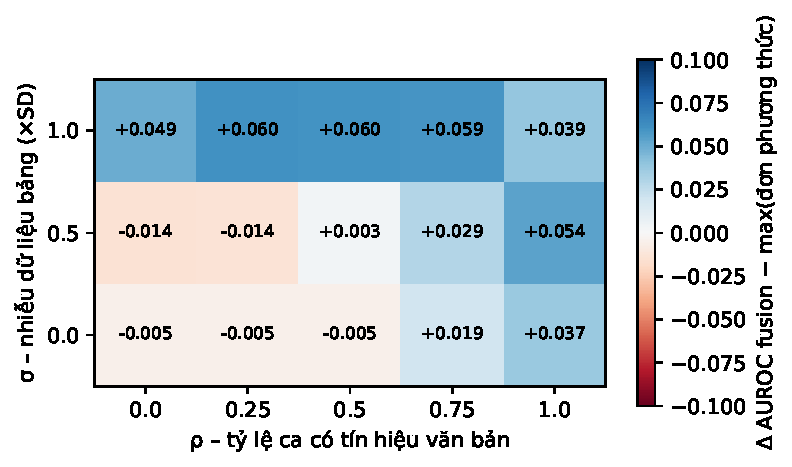
\includegraphics[width=0.6\linewidth]{figures/generated/fig_rq3_heatmap.pdf}
  \caption{RQ3 -- $\Delta$ AUROC giữa cross-attention và mô hình đơn phương thức tốt hơn theo tỷ lệ ca có tín hiệu văn bản ($\rho$) và mức nhiễu dữ liệu bảng ($\sigma$).}
  \label{fig:rq3}
\end{figure}}{Kết quả RQ3 chưa được sinh.}

\subsection{RQ4 -- Hiệu chuẩn, lợi ích ròng và độ bền}
\textbf{Hiệu chuẩn.} Temperature scaling giảm ECE của mô hình triển khai từ \eceUncal{} xuống \eceTemp{} (Bảng~\ref{tab:calibration}, Hình~\ref{fig:calibration}); vector scaling và isotonic khớp trên tập validation 273 ca không cải thiện thêm. \textbf{Không phương pháp nào đạt mục tiêu ECE $<0.05$} đã đặt ra.

% AUTO-GENERATED by scripts/export_latex_tables.py from results/registry.json. Do not edit.
\begin{table}[htbp]\centering\small
\caption{RQ4a -- Hiệu chuẩn mô hình triển khai (fit trên validation $N=273$, đo trên test $N=302$).}
\label{tab:calibration}
\begin{tabular}{@{}lcccccc@{}}\toprule
Phương pháp & ECE (10 bins) & CI 95\% & ECE (15, equal-mass) & Classwise ECE & Brier & NLL \\ \midrule
Không hiệu chuẩn & 0.079 & [0.050; 0.127] & 0.111 & 0.085 & 0.326 & 0.700 \\
Temperature scaling & 0.077 & [0.050; 0.124] & 0.121 & 0.099 & 0.321 & 0.653 \\
Vector scaling & 0.098 & [0.058; 0.148] & 0.136 & 0.089 & 0.360 & 0.935 \\
Isotonic (one-vs-rest) & 0.094 & [0.063; 0.148] & 0.171 & 0.096 & 0.393 & 2.315 \\
\bottomrule\end{tabular}\end{table}


\begin{figure}[htbp]
  \centering
  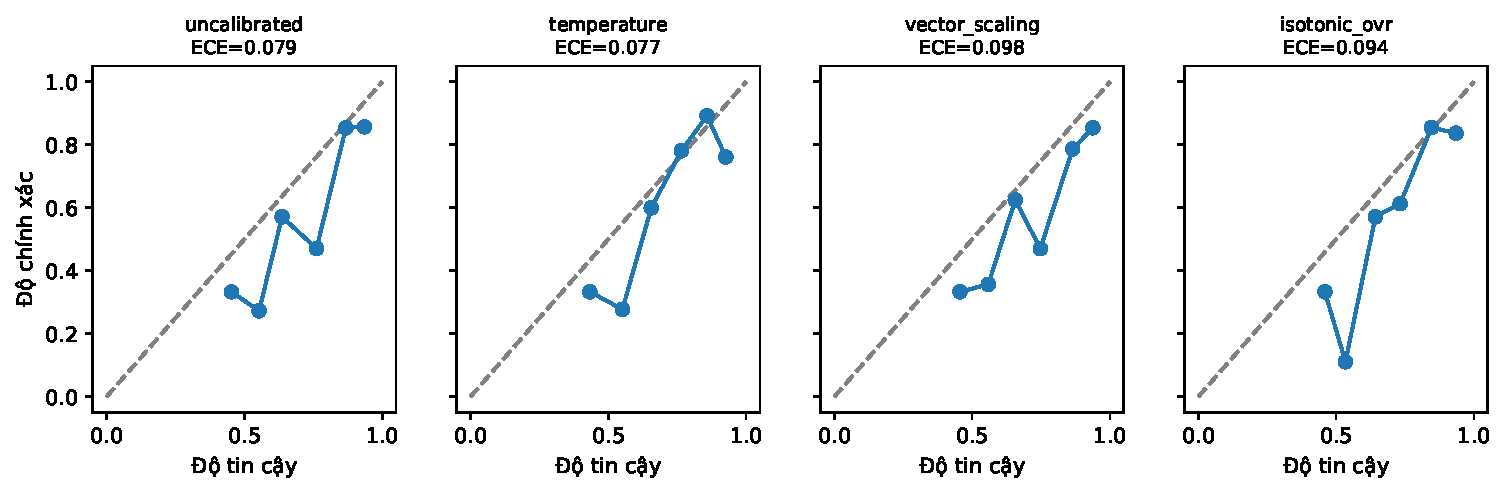
\includegraphics[width=\linewidth]{figures/generated/fig_calibration.pdf}
  \caption{Biểu đồ độ tin cậy của mô hình triển khai trên tập test theo bốn phương pháp hiệu chuẩn.}
  \label{fig:calibration}
\end{figure}

\textbf{Lợi ích ròng (DCA).} Với bài toán suy tim one-vs-rest, mọi mô hình đều có net benefit cao hơn chiến lược ``can thiệp tất cả'' và ``không can thiệp'' trên toàn dải $p_t\in[0.05;0.30]$ (Bảng~\ref{tab:dca}, Hình~\ref{fig:dca}); khoảng tin cậy bootstrap giữa các mô hình chồng lấn. Tỷ lệ suy tim trong tập test là 35.1\%, cao hơn nhiều so với chăm sóc ban đầu, và cả 106 bản ghi suy tim trong test đến từ \emph{một} bệnh nhân Synthea gốc; vì vậy DCA ở đây chỉ minh hoạ phương pháp, giá trị net benefit không ngoại suy được và không đủ để kết luận về lợi ích lâm sàng.

% AUTO-GENERATED by scripts/export_latex_tables.py from results/registry.json. Do not edit.
\begin{table}[htbp]\centering\small
\caption{RQ4b -- Phân tích đường cong quyết định, suy tim one-vs-rest (tỷ lệ hiện mắc test 35.1\%). Số can thiệp giảm ròng/100 BN $=(\text{NB}-\text{NB}_{\text{all}})(1-p_t)/p_t\times100$.}
\label{tab:dca}
\begin{tabular}{@{}lcccc@{}}\toprule
Mô hình & NB ($p_t$=0.10) & Giảm can thiệp/100 & NB ($p_t$=0.20) & Giảm can thiệp/100 \\ \midrule
Can thiệp tất cả & 0.279 & -- & 0.189 & -- \\
\textbf{Cross-attention (đóng băng)} & 0.345 & 59.6 & 0.344 & 61.9 \\
CatBoost & 0.339 & 54.0 & 0.341 & 60.9 \\
Bio\_ClinicalBERT (fine-tune) & 0.336 & 51.0 & 0.327 & 55.3 \\
Ensemble CatBoost + BERT-FT & 0.337 & 52.6 & 0.333 & 57.6 \\
Logistic Regression & 0.329 & 45.4 & 0.315 & 50.7 \\
\bottomrule\end{tabular}\end{table}


\begin{figure}[htbp]
  \centering
  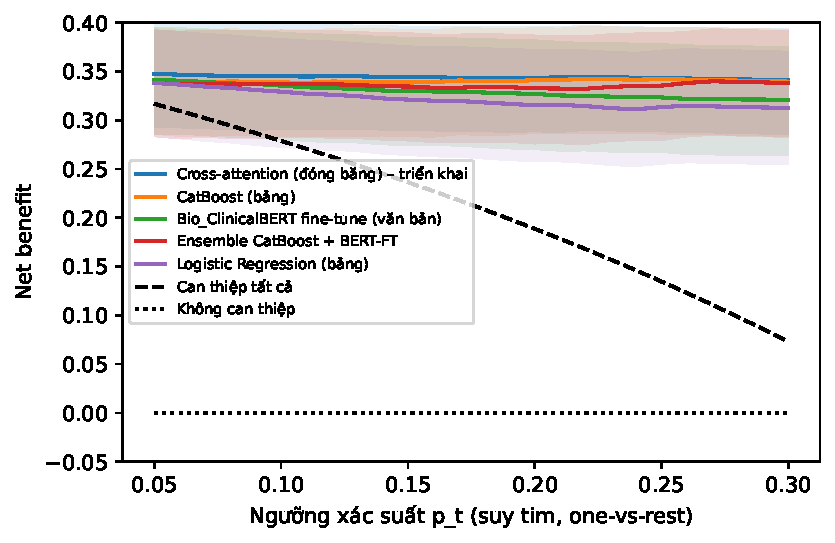
\includegraphics[width=0.75\linewidth]{figures/generated/fig_dca.pdf}
  \caption{Đường cong quyết định cho suy tim (one-vs-rest), dải mờ là CI 95\% bootstrap.}
  \label{fig:dca}
\end{figure}

\textbf{Thiếu dữ liệu lúc suy luận.} Khi thiếu ngẫu nhiên 10--50\% biến số, cross-attention suy giảm chậm hơn CatBoost (Bảng~\ref{tab:robustness}, Hình~\ref{fig:missing}) vì vẫn đọc được giá trị tương ứng trong ghi chú. Tuy nhiên khi mất toàn bộ dữ liệu bảng, AUROC của mô hình dung hợp giảm mạnh, trong khi BERT-FT không bị ảnh hưởng; khi mất văn bản, mô hình dung hợp thấp hơn CatBoost. Các mô hình được huấn luyện trên dữ liệu đầy đủ, không có kỹ thuật bỏ ngẫu nhiên phương thức (modality dropout); đây là hướng cải thiện trực tiếp.

% AUTO-GENERATED by scripts/export_latex_tables.py from results/registry.json. Do not edit.
\begin{table}[htbp]\centering\small
\caption{RQ4c -- Độ bền khi thiếu dữ liệu lúc suy luận (macro AUROC, trung bình qua seed). Mô hình được huấn luyện trên dữ liệu đầy đủ.}
\label{tab:robustness}
\begin{tabular}{@{}lccccc@{}}\toprule
Kịch bản & Cross-attn & CatBoost & LR bảng & BERT-FT & Ensemble \\ \midrule
Đầy đủ & 0.956 & 0.925 & 0.945 & 0.975 & 0.978 \\
Thiếu 10% biến số & 0.936 & 0.897 & 0.914 & 0.975 & 0.976 \\
Thiếu 30% biến số & 0.908 & 0.856 & 0.869 & 0.975 & 0.976 \\
Thiếu 50% biến số & 0.888 & 0.823 & 0.822 & 0.975 & 0.977 \\
Mất toàn bộ bảng & 0.678 & 0.500 & 0.500 & 0.975 & 0.975 \\
Mất văn bản & 0.902 & 0.925 & 0.945 & 0.501 & 0.925 \\
\bottomrule\end{tabular}\end{table}


\begin{figure}[htbp]
  \centering
  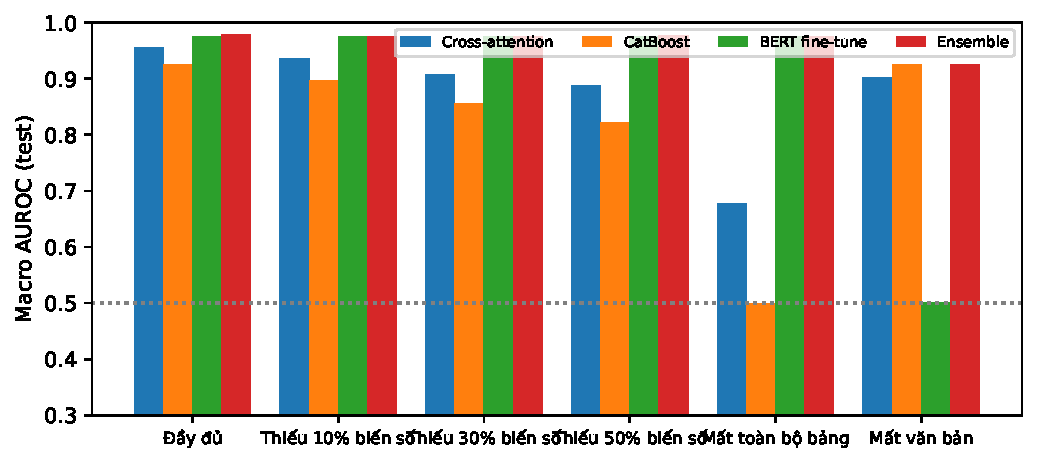
\includegraphics[width=0.85\linewidth]{figures/generated/fig_missing_modality.pdf}
  \caption{Macro AUROC khi thiếu dữ liệu lúc suy luận (trung bình qua seed).}
  \label{fig:missing}
\end{figure}

\textbf{Độ bền nội bộ.} Bảng~\ref{tab:generalization} báo cáo 5-fold grouped CV (post-hoc) và temporal split. Trong grouped CV, cross-attention có AUROC trung bình cao nhất và độ lệch chuẩn nhỏ nhất; ngược lại, trên temporal split cross-attention giảm còn \tmpXattn{} trong khi CatBoost giữ \tmpCatBoost. Hai kết quả trái chiều này cho thấy xếp hạng giữa các mô hình không ổn định trên đoàn hệ có ít bệnh nhân gốc. Đây là kiểm tra trên cùng đoàn hệ bán tổng hợp, \emph{không} phải ngoại kiểm.

% AUTO-GENERATED by scripts/export_latex_tables.py from results/registry.json. Do not edit.
\begin{table}[htbp]\centering\small
\caption{Độ bền nội bộ: (a) 5-fold grouped CV \textbf{post-hoc} trên 2.000 ca (trung bình $\pm$ SD qua fold, seed 42); (b) temporal split theo nhóm nguồn (dấu thời gian tổng hợp). Không phải ngoại kiểm.}
\label{tab:generalization}
\begin{tabular}{@{}lccc@{}}\toprule
Mô hình & (a) Grouped CV & (b) Temporal [CI 95\%] & Strict (cùng seed) \\ \midrule
Logistic Regression & 0.909 $\pm$ 0.021 & -- -- & -- \\
CatBoost & 0.892 $\pm$ 0.036 & 0.936 [0.916; 0.954] & 0.926 \\
TF-IDF + LR & 0.904 $\pm$ 0.084 & 0.904 [0.876; 0.928] & 0.917 \\
Bio\_ClinicalBERT (đóng băng) & 0.833 $\pm$ 0.064 & 0.879 [0.845; 0.909] & 0.904 \\
Bio\_ClinicalBERT (fine-tune) & 0.894 $\pm$ 0.148 & -- -- & -- \\
\textbf{Cross-attention (đóng băng)} & 0.949 $\pm$ 0.016 & 0.879 [0.850; 0.906] & 0.958 \\
Ensemble CatBoost + BERT-FT & 0.931 $\pm$ 0.066 & -- -- & -- \\
\bottomrule\end{tabular}\end{table}


\subsection{Phân nhóm và phân tích lỗi}
Bảng~\ref{tab:fairness} trình bày hiệu năng theo phân nhóm. Nhiều phân nhóm thiếu hẳn một số lớp (ví dụ không có ca suy tim nữ, không có người đang hút thuốc trong tập test) do cách sinh dữ liệu tổng hợp, nên AUROC chỉ tính trên các lớp có mặt và không thể diễn giải như đánh giá công bằng. Ma trận nhầm lẫn (Hình~\ref{fig:confusion}) cho thấy nhầm lẫn tập trung ở cặp hen -- viêm phổi và hen -- COPD; chi tiết 30 ca nhầm lẫn có độ tin cậy cao nhất nằm trong \texttt{results/registry.json} (\texttt{error\_analysis}) và \texttt{docs/06\_ERROR\_ANALYSIS\_AND\_CLINICAL\_DISCREPANCIES.md}. Hai ca minh hoạ từ Giai đoạn 1 đều được mô hình triển khai dự đoán đúng: \texttt{PT-0044} (hen) và \texttt{PT-0254} (COPD).

% AUTO-GENERATED by scripts/export_latex_tables.py from results/registry.json. Do not edit.
\begin{table}[htbp]\centering\small
\caption{Phân nhóm (mô hình triển khai, CI 95\% bootstrap). Dữ liệu tổng hợp: chỉ mô tả hành vi pipeline, không phải công bằng trên bệnh nhân thật.}
\label{tab:fairness}
\begin{tabular}{@{}lccc@{}}\toprule
Phân nhóm & $N$ & Macro AUROC [CI 95\%] & Macro-F1 [CI 95\%] \\ \midrule
gender M & 206 & 0.951 [0.926; 0.971] & 0.621 [0.555; 0.684] \\
gender F & 96 & 0.924 [0.850; 0.977] & 0.855 [0.778; 0.921] \\
age under 65 & 237 & 0.914 [0.893; 0.933] & 0.676 [0.642; 0.703] \\
age 65 and older & 65 & 0.814 [0.685; 0.936] & 0.515 [0.441; 0.591] \\
smoking NEVER & 160 & 0.924 [0.894; 0.950] & 0.639 [0.567; 0.709] \\
smoking FORMER & 142 & 0.966 [0.924; 0.996] & 0.857 [0.758; 0.941] \\
smoking CURRENT & 0 & -- -- & -- -- \\
\bottomrule\end{tabular}\end{table}


\begin{figure}[htbp]
  \centering
  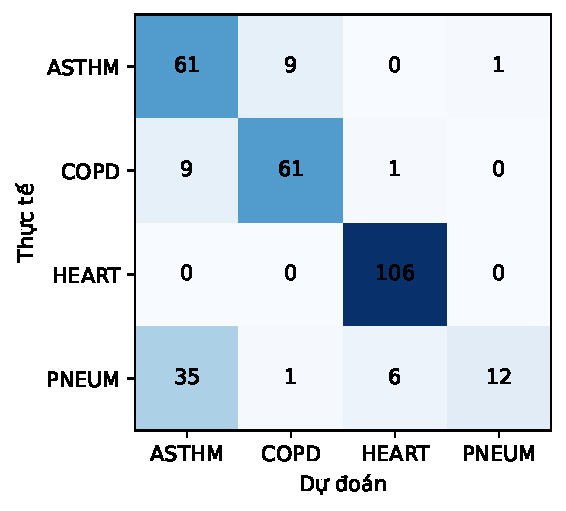
\includegraphics[width=0.45\linewidth]{figures/generated/fig_confusion_matrix.pdf}
  \caption{Ma trận nhầm lẫn của mô hình triển khai trên tập test strict.}
  \label{fig:confusion}
\end{figure}

\subsection{RQ5 -- Truy xuất và neo bằng chứng}
Kết quả đánh giá truy xuất phác đồ và neo bằng chứng được trình bày tại Mục~\ref{sec:multi_agent_rag} (Bảng~\ref{tab:rag_eval}).
